\documentclass[a4paper]{article}
\usepackage[utf8]{inputenc}
\usepackage[english]{babel}
\usepackage{moreverb}
\usepackage{graphicx}
\title{Assignment 1 \\ EDA132 Applied Artificial Intelligence}
\date{\today}
\author{Fredrik Paulsson \\ dat11fp1@student.lu.se \and Shan Senanayake \\ dat11sse@student.lu.se}
%\setcounter{secnumdepth}{5}
%\setcounter{tocdepth}{5}
\begin{document}
\maketitle
%\tableofcontents


\section{Introduction}
In this assignment we had the task to construct a program with a playable Othello game and an AI bot as the opponent. The game is played with ASCII art over the console. The program is written in Java and consists of three classes which are OthelloGame, OthelloAI and OthelloMain. Theses classes will be further explained later in this report. \\

\section{OthelloGame}
This class represents the game board and all the rules for the game. It consists of two constructors, seven public methods and a couple of private methods. In addition to this it also contains field and static variables that are used throughout the class to have a more dynamic use of variables.
\subsection{Fields}
\begin{description}
\item[\texttt{public static final char L}] This character represents the 'Light' player outside of the class and board.
\item[\texttt{public static final char D}] This character represents the 'Dark' player outside of the class and board.
\item[\texttt{private static final char E}] This character represents an empty space on the board outside of the class and board.
\item[\texttt{private static final char V}] This character represents a valid move on the board outside of the class and board.
\item[\texttt{private static final int EMPTY}] This int represents an empty space on the board in the board matrix, this variable has the value 0 to make the heuristic function easier to compute. 
\item[\texttt{private static final int LIGHT}] This int represents the 'Light' player on the board in the board matrix, this variable has the value 1 to make the heuristic function easier to compute. 
\item[\texttt{private static final int DARK}] This int represents the 'Dark' player on the board in the board matrix, this variable has the value -1 to make the heuristic function easier to compute. 
\item[\texttt{private int[][] board}] Represents the board of the game.
\item[\texttt{private int player}] Represents which player has the current turn.
\item[\texttt{private int HashMap<String, HashSet<Integer[]>> validMoves}] Represents the valid moves which can be made by the current player, and which tiles will be flipped when that move is made.
\end{description} 
\subsection{Constructors}
OthelloGame has two constructors one public constructur and one private. The public constructor is used to initiate the game. The private constructor is used to create a certain game in a certain state this is used to make a copy of an already existing game.
\subsection{Methods}
This class has a lot of methodes (around 16-17 both private and public methodes), to cut down the unnecessary methodes only the most important parts revolving the AI are included in this report. The other methodes handle prints, making moves and conversions (between print format and such) as well as getters and setters that are needed for the AI and starting the program.  
\begin{description}
\item[\texttt{private void findValidMoves()}] This method finds all the valid moves the current player can make, as well as finds all the tiles that will be flipped. And sets this as the \texttt{validMoves} map.
\item[\texttt{private HashSet<Integer[]> checkDirection(int x, int y, int incX, int incY)}] The method \texttt{findValidMoves()} uses this method to check in a certain direction which tiles will be flipped, if a tile of the current player is picked. The direction is indicated by the \texttt{incX} and \texttt{incY} parameters.
\item[\texttt{public int sumScore()}] This methods is the heuristic function currently being used, it sums the whole \texttt{board} variable, and returns the value gained.
\end{description} 

\section{OthelloAI}
OthelloAI is the class that implements the AI part of the game. It interacts with the OthelloGame to be able to present a move that is as good as possible. This is works by supplying a maximum processing time for the AI to respond with a move. 

\subsection{Algorithms}
The algorithm used to determine the best move is the Minimax algorithm with Alpha-Beta pruning implemented. The Minimax algorithm is an algorithm which considers all moves for that remains before the game is finished. It looks at all moves possible in the current turn of the game and for all those moves the next possible moves and so on. This means that all possible moves are tried out and finally one move is selected as the best. In order to select this move the algorithm always assume that the opponent makes the worst move from the AI point of view. Therefore the algorithm assumes the opponent makes the move which has the minimum of value of the heuristic function and then the algorithm selects the move that maximizes the heuristic function.

As can be realized it is extremely demanding to consider all possible moves for all possible turns in the game. To mitigate this we have done two optimizations. The first one is Alpha-Beta pruning which means that we do not consider moves which cannot be better than moves that has already been considered. However even with Alpha-Beta pruning the algorithm might take quite some time to compute the best possible move. To make the algorithm run in a reasonable amount of time we have given the AI a time limit for which it can run the algorithm. If the time limit is reached then return the best possible move from that standpoint. Since the Minimax algorithm runs a Depth first search, the resulting time limit might mean that the algorithm is still stuck in one branch and has not yet evaluated the next branches. To fix this we have done an iterative DFS. We run the Minimax algorithm one layer at a time, and between each layer we check if the time limit is reach, if not try to go one layer deeper. This will make a valid best move for the given time limit. \\

The Minimax algorithm can be visualized as a decision tree. Such a tree is diplayed in figure \ref{minimax}. Level 1 holds the moves that are possible for the algorithm to decide between and level 0 is the move that is selected. The values displayed in the nodes are the heuristic function's values. The algorithm has to select the move which has the maximum value in odd levels of the tree and it selects the moves with the minimum values in even levels of the tree. Alpha-Beta pruning works in the following manner. If the right hand side of level 1 has been calculated the left hand side does not need to because when looking calculating the values of the children to the left hand side and the value -10 has been calculated no more work has to be done. This is because the values are minimized on level 2 in the tree and therefore it is guaranteed that the result of the left hand side on level 1 is at the greatest -10, but we already had a better value, -7, for the right hand side. Using this technique makes it possible to remove several nodes from from consideration and therefore remove costly operations.

\begin{figure}[h!]
  \centering
    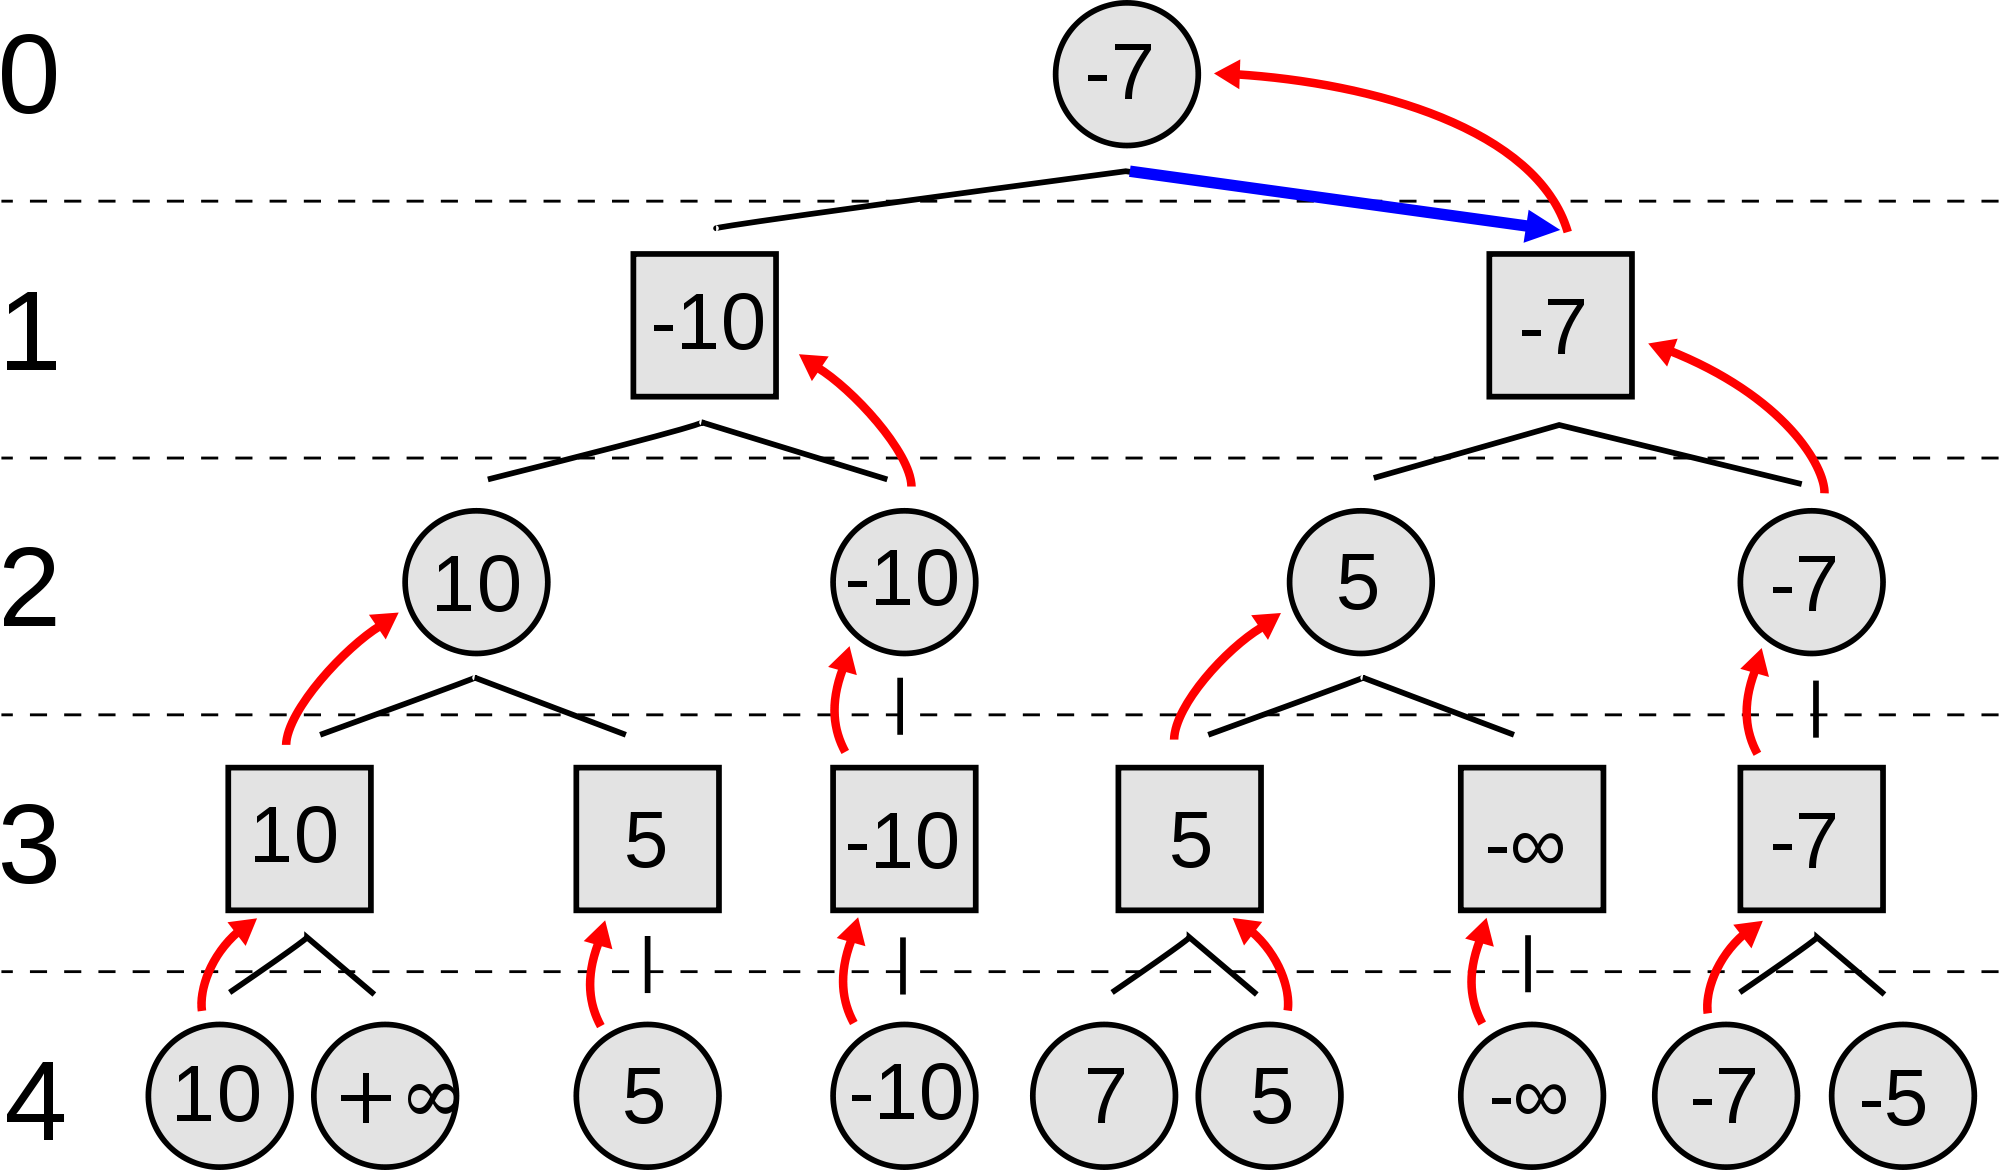
\includegraphics[width=1\textwidth]{Minimax.png}
  \caption{Minimax decision tree. Source: http://en.wikipedia.org/wiki/File:Minimax.svg}
  \label{minimax}
\end{figure}

\subsection{Heuristics}
As described above a position of the game board has the value of 1, -1 or 0 depending on if the light or dark player owns the position or if the position is empty. We have decided to let the AI play as the player whose game piece is represented by the value 1. The opponent is thus represented as the value -1. Because of this we chose the heuristic function to be the sum of all the positions on the board. This means that the AI wishes to have as high a value as possible of this function because this means that it is the leading player.

Chosing the heuristic function like this is very natural for the Minimax algorithm. The AI wants to maximize it's lead and therefore it maximizes the heuristic function. It also assumes that the opponent selects the move which maximizes the opponents lead and thus minimizing the heuristic function.

The herustic function we have selected also has one big advantage and that is that it can be calculated exactly even though the game has not yet been finished. Therefore it is not essential for the Minimax algorithm to reach the terminal nodes before having values on the different moves. Of, course only considered moves will contribute to the heuristic function this way.



\section{OthelloMain}

\section{Running Instructions}
The three .java files containing the classes described above are located in a package called othello placed on /h/d9/v/dat11fp1/TAI/othello on the student computer system. It is simply to compile the java files in the package and then run OthelloMain from outside that package. For example if the current directory is /h/d9/dat11fp1/TAI the following command will compile the files: \texttt{javac othello/*.java}. After compiling the program can be run with the following command: \texttt{java othello.OthelloMain}.

\begin{thebibliography}{1}
\bibitem{wikipedia}
http://en.wikipedia.org
\end{thebibliography}
\end{document}